
%%erstellt mit https://www.mathcha.io/editor

\tikzset{every picture/.style={line width=0.75pt}} %set default line width to 0.75pt        

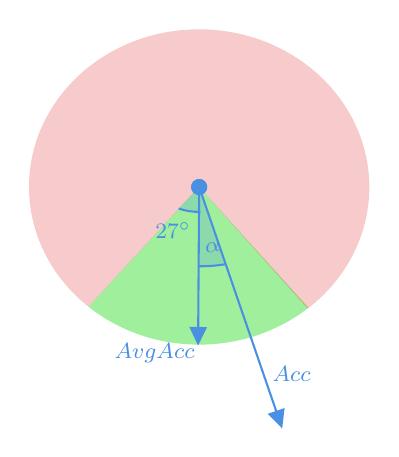
\begin{tikzpicture}[x=0.75pt,y=0.75pt,yscale=-1,xscale=1]
%uncomment if require: \path (0,410.90625); %set diagram left start at 0, and has height of 410.90625

%Shape: Arc [id:dp6141700786507858] 
\draw  [draw opacity=0][fill={rgb, 255:red, 81; green, 226; blue, 74 }  ,fill opacity=0.55 ] (374.18,293.16) .. controls (359.81,304.36) and (341.22,311.06) .. (320.96,310.93) .. controls (300.8,310.81) and (282.38,303.95) .. (268.17,292.67) -- (321.44,234.95) -- cycle ; \draw  [color={rgb, 255:red, 226; green, 74; blue, 79 }  ,draw opacity=0 ] (374.18,293.16) .. controls (359.81,304.36) and (341.22,311.06) .. (320.96,310.93) .. controls (300.8,310.81) and (282.38,303.95) .. (268.17,292.67) ;
%Straight Lines [id:da39478853698383154] 
\draw [color={rgb, 255:red, 74; green, 144; blue, 226 }  ,draw opacity=1 ]   (321.5,235) -- (321,308.36) ;
\draw [shift={(320.97,311.36)}, rotate = 270.39] [fill={rgb, 255:red, 74; green, 144; blue, 226 }  ,fill opacity=1 ][line width=0.08]  [draw opacity=0] (8.93,-4.29) -- (0,0) -- (8.93,4.29) -- cycle    ;
\draw [shift={(321.5,235)}, rotate = 90.39] [color={rgb, 255:red, 74; green, 144; blue, 226 }  ,draw opacity=1 ][fill={rgb, 255:red, 74; green, 144; blue, 226 }  ,fill opacity=1 ][line width=0.75]      (0, 0) circle [x radius= 3.35, y radius= 3.35]   ;
%Shape: Arc [id:dp5049979934092728] 
\draw  [draw opacity=0][fill={rgb, 255:red, 226; green, 74; blue, 77 }  ,fill opacity=0.29 ] (268.17,292.67) .. controls (250.51,278.62) and (239.38,257.74) .. (239.52,234.48) .. controls (239.79,192.52) and (276.7,158.73) .. (321.98,159.02) .. controls (367.25,159.3) and (403.74,193.55) .. (403.48,235.52) .. controls (403.33,258.91) and (391.79,279.76) .. (373.77,293.59) -- (321.5,235) -- cycle ; \draw  [color={rgb, 255:red, 226; green, 74; blue, 79 }  ,draw opacity=0 ] (268.17,292.67) .. controls (250.51,278.62) and (239.38,257.74) .. (239.52,234.48) .. controls (239.79,192.52) and (276.7,158.73) .. (321.98,159.02) .. controls (367.25,159.3) and (403.74,193.55) .. (403.48,235.52) .. controls (403.33,258.91) and (391.79,279.76) .. (373.77,293.59) ;
%Shape: Arc [id:dp7716732689668444] 
\draw  [draw opacity=0][fill={rgb, 255:red, 74; green, 144; blue, 226 }  ,fill opacity=0.22 ] (322.06,247) .. controls (321.85,247) and (321.64,247) .. (321.42,247) .. controls (317.86,246.98) and (314.51,246.38) .. (311.63,245.35) -- (321.5,235) -- cycle ; \draw  [color={rgb, 255:red, 74; green, 144; blue, 226 }  ,draw opacity=1 ] (322.06,247) .. controls (321.85,247) and (321.64,247) .. (321.42,247) .. controls (317.86,246.98) and (314.51,246.38) .. (311.63,245.35) ;
%Straight Lines [id:da07556207680782712] 
\draw [color={rgb, 255:red, 74; green, 144; blue, 226 }  ,draw opacity=1 ]   (321.5,235) -- (360.52,348.48) ;
\draw [shift={(361.5,351.32)}, rotate = 251.01999999999998] [fill={rgb, 255:red, 74; green, 144; blue, 226 }  ,fill opacity=1 ][line width=0.08]  [draw opacity=0] (8.93,-4.29) -- (0,0) -- (8.93,4.29) -- cycle    ;
\draw [shift={(321.5,235)}, rotate = 71.02] [color={rgb, 255:red, 74; green, 144; blue, 226 }  ,draw opacity=1 ][fill={rgb, 255:red, 74; green, 144; blue, 226 }  ,fill opacity=1 ][line width=0.75]      (0, 0) circle [x radius= 3.35, y radius= 3.35]   ;
%Shape: Arc [id:dp542059610762009] 
\draw  [draw opacity=0][fill={rgb, 255:red, 74; green, 144; blue, 226 }  ,fill opacity=0.22 ] (334.22,272.18) .. controls (330.14,272.86) and (325.88,273.21) .. (321.49,273.18) .. controls (321.41,273.18) and (321.32,273.18) .. (321.24,273.18) -- (321.73,235.77) -- cycle ; \draw  [color={rgb, 255:red, 74; green, 144; blue, 226 }  ,draw opacity=1 ] (334.22,272.18) .. controls (330.14,272.86) and (325.88,273.21) .. (321.49,273.18) .. controls (321.41,273.18) and (321.32,273.18) .. (321.24,273.18) ;

% Text Node
\draw (300,315) node  [font=\footnotesize,color={rgb, 255:red, 74; green, 144; blue, 226 }  ,opacity=1 ]  {$AvgAcc$};
% Text Node
\draw (309,256) node  [font=\footnotesize,color={rgb, 255:red, 74; green, 144; blue, 226 }  ,opacity=1 ]  {$27^{\circ}$};
% Text Node
\draw (366,325) node  [font=\footnotesize,color={rgb, 255:red, 74; green, 144; blue, 226 }  ,opacity=1 ]  {$Acc$};
% Text Node
\draw (328,264) node  [font=\footnotesize,color={rgb, 255:red, 74; green, 144; blue, 226 }  ,opacity=1 ,rotate=-349.43]  {$\alpha $};


\end{tikzpicture}\\
